%%%%%%%%%%%%%%%%%%%%%%%%
%
% $Author: Sadegh Naderi $
% $Datum: 2023-06-29  $
% $Pfad: BA23-02-Sales-Predictor/report/Contents/en/Packages.tex $
% $Version: 1.0 $
% $Reviewed by: Deepti, Sadegh and Raunak $
% $Review Date: 2023-06-30 $
%
%%%%%%%%%%%%%%%%%%%%%%%%




\chapter{Application}


\section{Description}
PyCharm Community is an integrated development environment (IDE) specifically designed for Python programming. It is developed by JetBrains and is available as a free and open-source software. PyCharm Community provides a comprehensive set of features and tools to enhance the productivity of Python developers.

The application offers a user-friendly interface and a powerful code editor with intelligent code completion, code inspections, and error highlighting, which helps developers write clean and efficient Python code. It also supports various Python frameworks and libraries, making it suitable for a wide range of Python projects.

PyCharm Community includes features like version control integration (e.g., Git, Mercurial), debugging capabilities, unit testing support, and project management tools. It allows developers to easily navigate through code, refactor code snippets, and analyze project dependencies. The IDE also offers a rich set of plugins to extend its functionality according to specific project requirements.

\subsection{Pick the ideal PyCharm for you}
PyCharm comes in two versions:
\begin{enumerate}
	\item PyCharm Community (free and open-source): Designed for intelligent Python development, it offers a range of features such as code assistance, refactorings, visual debugging, and integration with version control systems.
	\item PyCharm Professional (paid): Geared towards professional Python, web, and data science development, it encompasses all the features of PyCharm Community along with additional capabilities. These include advanced code assistance, refactorings, visual debugging, version control integration, remote configurations, deployment features, support for popular web frameworks like Django and Flask, database support, scientific tools (including Jupyter notebook support), and big data tools.
\end{enumerate}

The version of Pycharm used is pycharm Community Edition 2022.3.3.


\section{OS/Interfaces/Protocols}
PyCharm Community is a cross-platform application that runs on major operating systems, including Windows, macOS, and Linux. It provides a consistent user experience across different platforms and supports a wide range of Python versions.

The application offers a graphical user interface (GUI) for easy interaction with developers. It provides a set of intuitive menus, toolbars, and panels to access various features and functionalities. PyCharm Community integrates with popular version control systems, such as Git, Mercurial, and Subversion, allowing seamless collaboration and code management.

PyCharm Community supports various protocols for remote development, including SSH, FTP, and SFTP. It enables developers to work on remote Python projects and interact with remote servers directly from within the IDE.

To ensure optimal performance, please review the system requirements outlined below:

\begin{table}[h!]
	\centering
	\caption{PyCharm System Requirements}
	\label{tab:system-requirements}
	\begin{tabular}{|p{3cm}|p{4cm}|p{4cm}|}
		\hline
		\textbf{Requirement} & \textbf{Minimum} & \textbf{Recommended} \\ \hline
		RAM & 4 GB of free RAM & 8 GB of total system RAM \\ \hline
		CPU & Any modern CPU & Multi-core CPU. PyCharm supports multithreading for different operations and processes, making it faster the more CPU cores it can use. \\ \hline
		Disk space & 3.5 GB & SSD drive with at least 5 GB of free space \\ \hline
		Monitor resolution & 1024×768 & 1920×1080 \\ \hline
		Operating system & Officially released 64-bit versions of: 
		- Microsoft Windows 10 1809 or later
		- Windows Server 2019 or later
		- macOS 10.15 or later
		- Any Linux distribution that supports Gnome, KDE, or Unity DE
		PyCharm is not available for Linux distributions without GLIBC 2.27 or later.
		Pre-release versions are not supported. & Latest 64-bit version of Windows, macOS, or Linux (e.g., Debian, Ubuntu, or RHEL) \\ \hline
	\end{tabular}
\end{table}


\subsection{Interface of PyCharm}

When you launch PyCharm for the first time or when no projects are open, you will be greeted with the Welcome screen. This screen serves as the main entry point into the IDE and offers options for creating or opening a project, checking out a project from version control, viewing documentation, and configuring the IDE.

Once a project is opened, the main window is divided into several logical areas. Let's take a closer look at the key UI elements in this interface (See Figure \ref{PyCharm_interface}):



\begin{center}
	\begin{figure}[h!]
		\begin{center}
			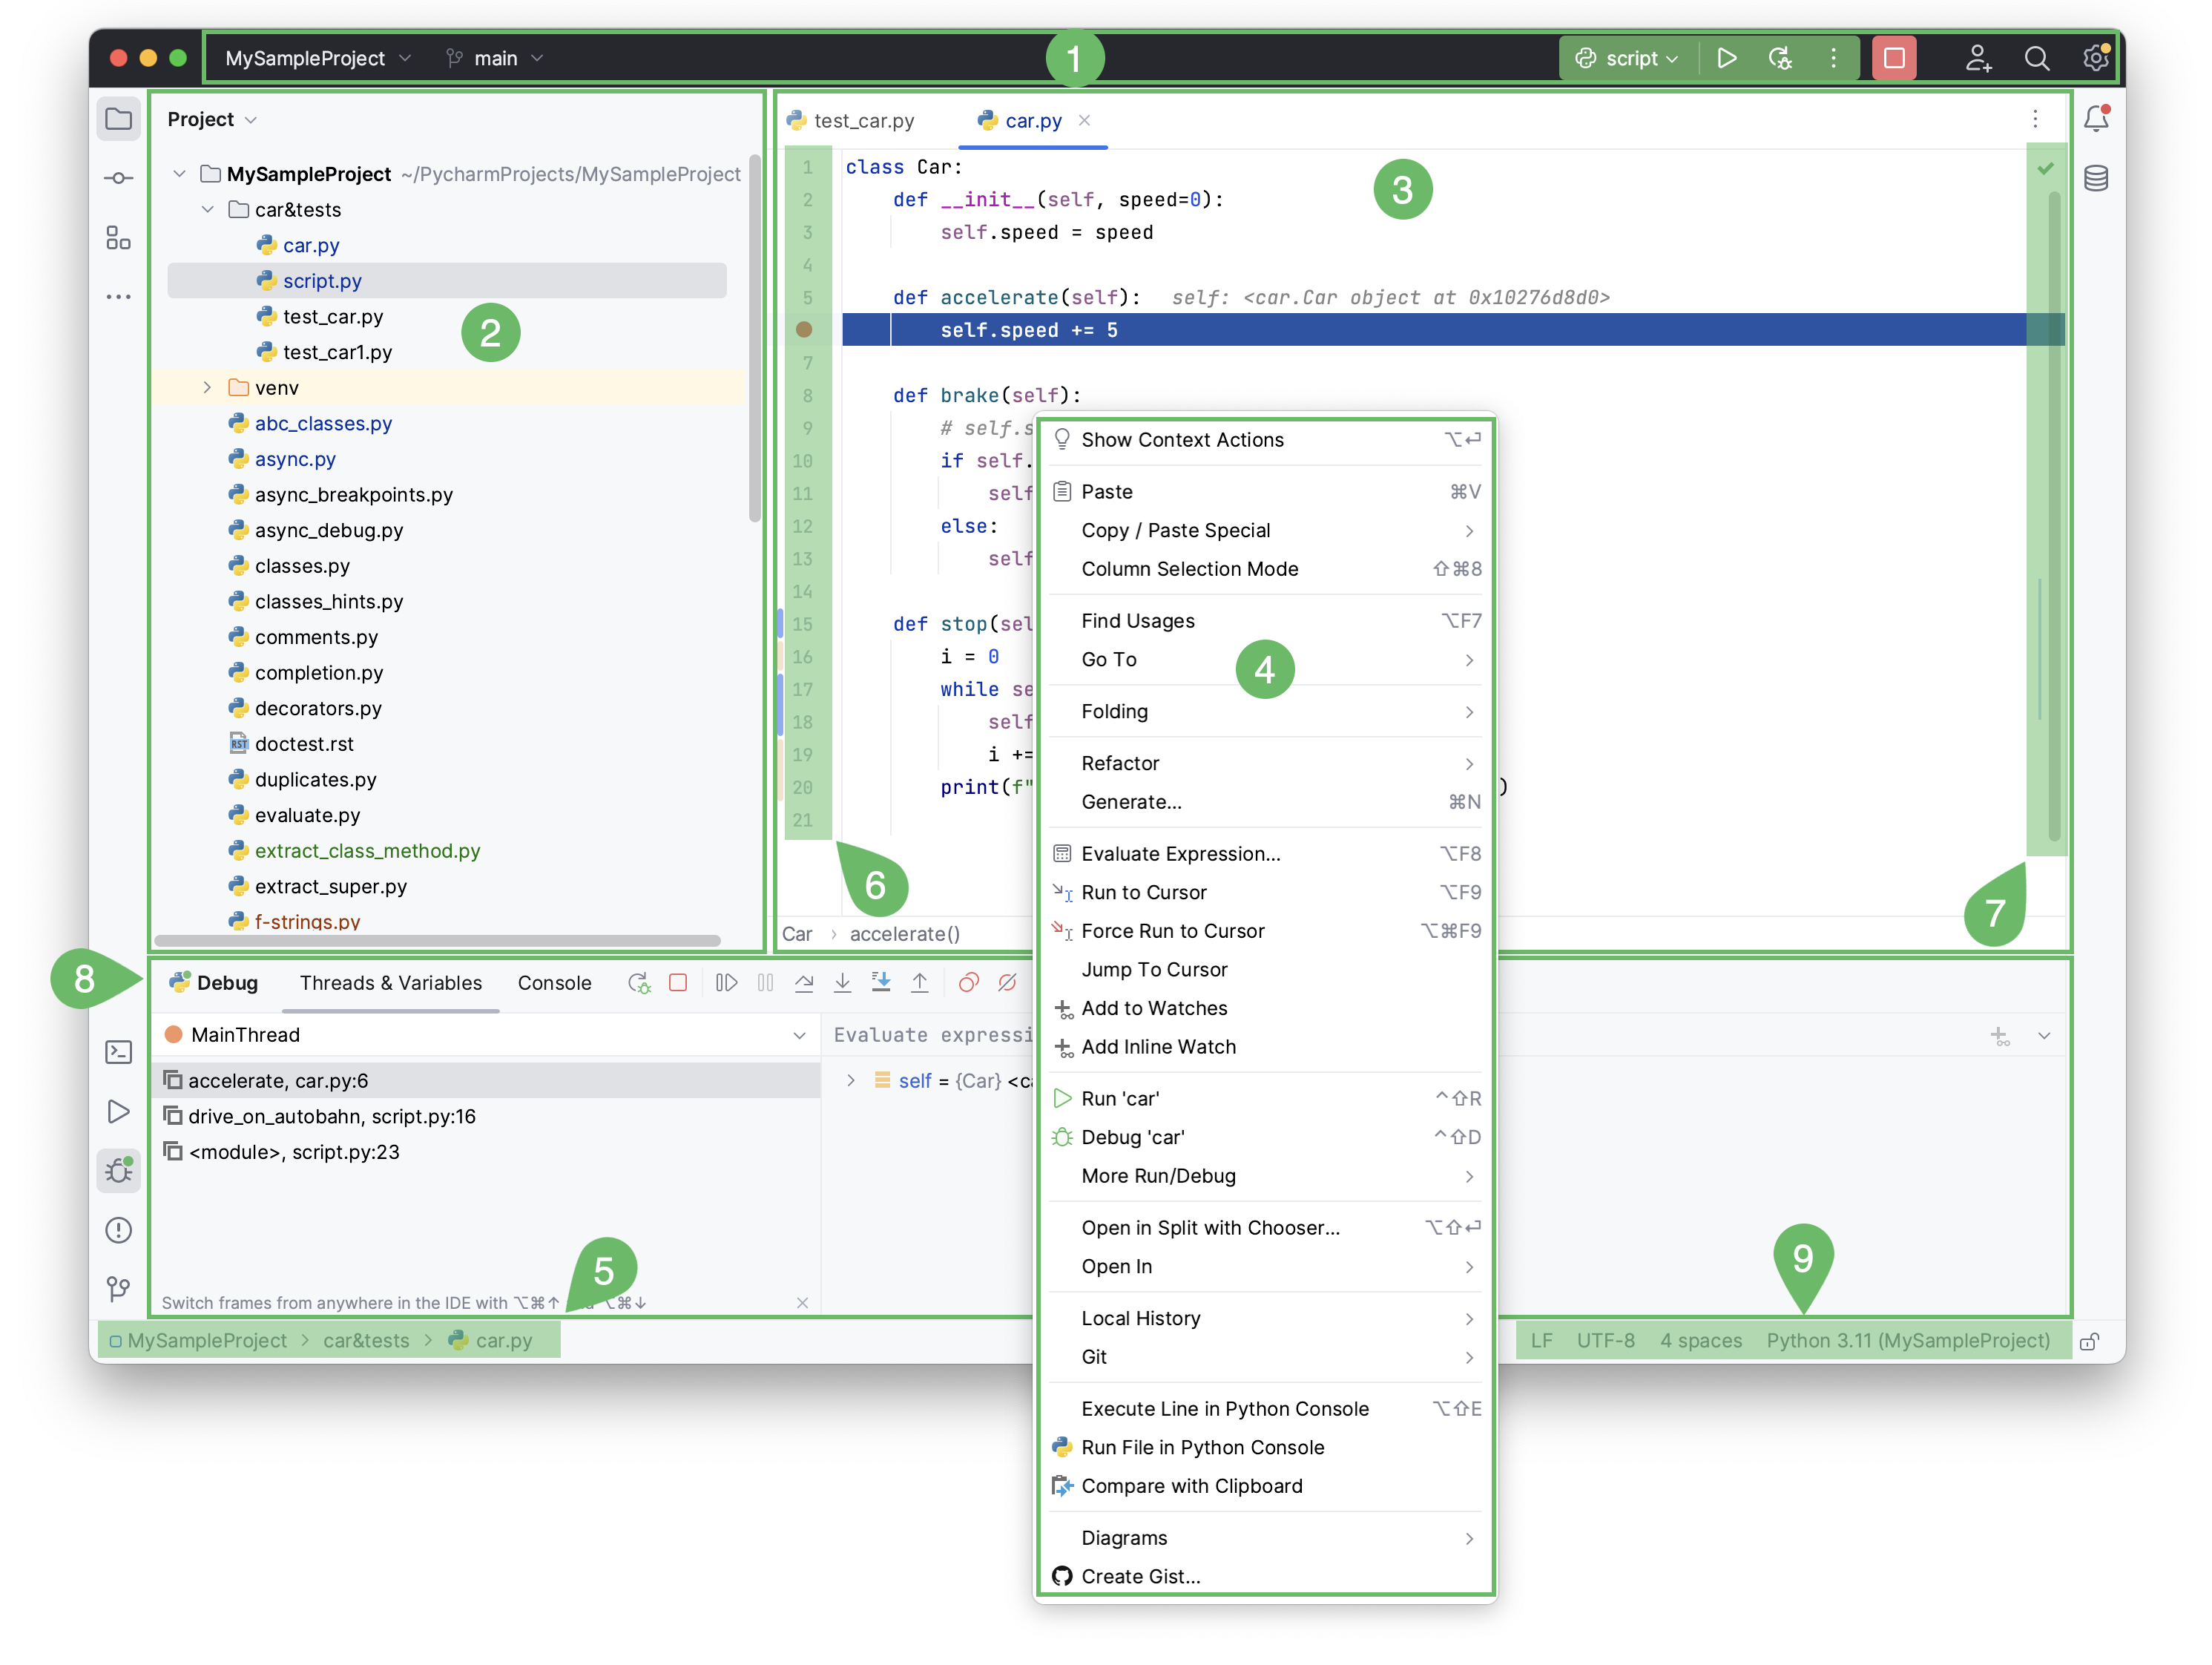
\includegraphics[height=90mm, width=130mm]{Images/pyMainWindowOverview.png}
		\end{center}
		\caption{PyCharm interface \cite{JetBrains:2023}}\label{PyCharm_interface}
	\end{figure}
\end{center}

\begin{enumerate}
	\item The window header contains a set of widgets that provide quick access to popular actions such as managing projects, version control, and running applications. It also provides shortcuts to features like Code With Me collaboration, Search Everywhere, and Settings.
	\item The Project tool window, located on the left side, displays your project files and directory structure.
	\item The Editor, situated on the right side, is where you write your code. It features tabs for easy navigation between open files.
	\item Context menus appear when you right-click on an element in the interface or a code fragment, providing a list of available actions.
	\item The Navigation bar enables swift navigation through project folders and files.
	\item The Gutter, a vertical stripe next to the editor, displays breakpoints you have set and facilitates navigation through the code hierarchy, including going to definitions or declarations. It also shows line numbers and per-line version control system (VCS) history.
	\item The Scrollbar, positioned on the right side of the editor, allows you to scroll through your code. The indicator in the top right-hand corner indicates the overall status of code inspections for the entire file, as PyCharm continually monitors the quality of your code.
	\item Tool windows are specialized windows attached to the bottom and sides of the workspace. They provide access to various tasks such as project management, source code search and navigation, version control system integration, running, testing, debugging, and more.
	\item The Status bar provides information about the status of your project and the entire IDE. It displays warnings and information messages related to file encoding, line separators, inspection profiles, and other relevant details. Additionally, it offers quick access to Python interpreter settings.
\end{enumerate}


The specific layout and appearance of the PyCharm interface can be customized based on your preferences. You can adjust the arrangement of tool windows, enable/disable specific panels, and configure the overall look and feel according to your workflow.

\subsubsection{Debugging in PyCharm}


PyCharm offers powerful debugging capabilities to help developers fix issues in Python code. Key debugging methods include:

\begin{itemize}
	\item \textbf{Breakpoints}: Pause code execution at specific lines or conditions, allowing examination of variables and code flow.
	\item \textbf{Step Into}: Dive into the details of called functions or methods for in-depth inspection and tracking.
	\item \textbf{Step Over}: Execute the next line of code without entering function calls, ideal for high-level flow analysis.
	\item \textbf{Step Out}: Move out of the current function being debugged and continue from its caller.
	\item \textbf{Evaluate Expression}: Evaluate and inspect expressions or variables during runtime without modifying the code.
	\item \textbf{Watches}: Monitor variables or expressions in real-time during debugging to track changes.
	\item \textbf{Debug Console}: An interactive Python console for executing code, evaluating expressions, and checking variables.
\end{itemize}

By utilizing these debugging features, developers can efficiently identify and resolve issues, ensuring more robust applications.

\subsection{protocols}


In the context of PyCharm, protocols are used to enable communication and interaction with external systems or services. PyCharm supports several protocols that allow developers to work with different aspects of software development. Here are some common protocols supported by PyCharm:

\begin{itemize}
	\item \textbf{SSH (Secure Shell):} PyCharm supports the SSH protocol, which allows developers to securely access and manage remote systems. It enables remote development, deployment, and interaction with remote servers directly from within the IDE.
	
	\item \textbf{FTP (File Transfer Protocol):} PyCharm has support for FTP, which is used for transferring files between a local machine and a remote server. It enables developers to upload, download, and synchronize files with a remote server.
	
	\item \textbf{SFTP (SSH File Transfer Protocol):} SFTP is an extension of the SSH protocol that provides secure file transfer capabilities. PyCharm supports SFTP, allowing developers to securely transfer files to and from remote servers.
	
	\item \textbf{HTTP (Hypertext Transfer Protocol):} PyCharm integrates with HTTP, which is the protocol used for communication between web browsers and web servers. It allows developers to work with web applications, send HTTP requests, and handle HTTP responses.
	
	\item \textbf{HTTPS (HTTP Secure):} PyCharm supports HTTPS, which is the secure version of HTTP. It enables secure communication between the IDE and web servers, ensuring the confidentiality and integrity of data exchanged.
\end{itemize}

These are some of the protocols commonly used with PyCharm. However, it's worth noting that PyCharm's protocol support can be extended through plugins and additional integrations based on specific project requirements.

\section{Getting Started with a Project in PyCharm}

In PyCharm, all your development activities are carried out within the context of a project. A project serves as the foundation for various features such as coding assistance, bulk refactoring, and maintaining coding style consistency. To begin working on a project in PyCharm, you have two options: opening an existing project or creating a new one.

\subsection{Opening an Existing Project}

To open an existing project, follow these steps:

\begin{enumerate}
	\item Select the desired project from the list of recent projects on the Welcome screen. Alternatively, click on the "Open" button.
	\item If your project's source files already exist, you can choose the "Open" option from the File menu. Specify the directory where the source files are located. PyCharm will create a project based on your existing sources.
\end{enumerate}

\subsection{Creating a New Project}

To create a new project, use one of the following methods:

\begin{enumerate}
	\item From the main menu, go to File $>$ New Project.
	\item On the Welcome screen, click on "New Project".
\end{enumerate}

\textbf{Note:} In PyCharm Community edition, you can only create Python projects. However, PyCharm Professional edition offers additional options, including creating web framework projects.

When creating a new project, you must specify a Python interpreter that will execute the Python code within your project. Ensure that at least one Python installation is available on your machine.

PyCharm automatically sets up an isolated virtual environment (venv, pipenv, poetry, or Conda) for your new project. You have the flexibility to change or create new interpreters as you work. Additionally, PyCharm provides a Python Package tool window that allows you to preview installed packages for your interpreters and easily add new packages.

By following these steps, you can efficiently start a project in PyCharm and leverage its powerful features for Python development.


\section{Constraints}
\begin{enumerate}
	\item \textbf{Limited Features:} PyCharm Community Edition provides a subset of the features available in its commercial counterpart, PyCharm Professional Edition. While it includes many essential features for Python development, some advanced functionalities like remote development, database tools, web development frameworks, and support for other programming languages may be absent.
	
	\item \textbf{No Support for Some Python Frameworks:} PyCharm Community Edition may not have built-in support or dedicated features for certain Python frameworks or libraries. For example, Django support is available, but more specialized frameworks like Flask, Pyramid, or web2py may not have comprehensive tooling within the Community Edition.
	
	\item \textbf{No Customizable Themes:} Unlike the Professional Edition, PyCharm Community Edition does not provide the ability to customize the IDE's appearance or create custom color themes. Users are limited to the default theme provided by the IDE.
	
	\item \textbf{Limited Support for Version Control Systems:} While PyCharm Community Edition supports version control systems like Git, Mercurial, and Subversion, some advanced version control features may not be available. For instance, integration with issue trackers or more sophisticated code review tools might be missing.
	
	\item \textbf{Restricted Database Tools:} PyCharm Community Edition has limited support for database management tools compared to PyCharm Professional Edition. It may lack certain advanced features for working with databases or may not support certain database systems.
	
	\item \textbf{Reduced Performance Analysis Tools:} Advanced profiling and performance analysis tools, such as the CPU and memory profiler, are not available in PyCharm Community Edition. These tools can be beneficial for optimizing code performance.
\end{enumerate}

It's worth noting that despite these constraints, PyCharm Community Edition remains a powerful and feature-rich IDE for Python development. It caters to the needs of many developers, especially those working on smaller projects or with basic requirements. For more advanced features and functionality, the Professional Edition of PyCharm is available for purchase.

\subsection{Conclusions}
PyCharm Community is a feature-rich and user-friendly IDE for Python development. It provides a comprehensive set of tools, code editor enhancements, and project management features to streamline the development process. While it has some limitations compared to the Professional edition, PyCharm Community is a popular choice among Python developers, particularly those who require a free and open-source solution.

The application's intuitive interface and extensive functionality make it suitable for a wide range of Python projects, from simple scripts to complex applications. Its cross-platform support and integration with popular version control systems further enhance the development experience.

\section{Data}

\subsection{Quality}

The quality of data used by PyCharm Community is dependent on the project and its associated codebase. The IDE provides powerful code analysis features, such as code inspections and error highlighting, to improve code quality. It helps identify potential issues, such as syntax errors, unused variables, and code smells, enabling developers to maintain high code quality standards.

Furthermore, PyCharm Community integrates with static code analysis tools like Pylint and Flake8, providing additional support for enhancing code quality. These tools analyze the code for potential bugs, enforce coding standards, and offer suggestions for improvement. By leveraging static code analysis tools, developers can identify and address issues early in the development process, leading to higher code quality and fewer bugs in the final application.

\subsection{Quantity}

In addition to focusing on code quality, PyCharm Community also considers the quantity of data used in a project and its associated codebase. The IDE provides developers with tools and features to effectively manage and handle large codebases, ensuring scalability and efficiency.

PyCharm Community offers support for projects of varying sizes, from small scripts to large-scale applications. It provides features like intelligent code completion, navigation, and search capabilities that significantly enhance productivity when working with extensive codebases. These features enable developers to efficiently locate specific code snippets, navigate through different files and modules, and quickly understand the structure of the project.

Moreover, PyCharm Community integrates with version control systems like Git, enabling seamless collaboration and efficient handling of code changes. It allows developers to track modifications, merge code branches, and revert changes if necessary, ensuring the integrity and consistency of the codebase.

Additionally, PyCharm Community supports advanced refactoring options, which help developers optimize and restructure their codebase. This includes features like code extraction, renaming, and restructuring that enable developers to make large-scale code modifications with confidence, reducing the risk of introducing errors or inconsistencies.

By providing comprehensive support for managing large codebases, PyCharm Community empowers developers to handle projects of any size effectively. Its features and tools streamline development workflows, improve productivity, and ensure the quantity of code is manageable and maintainable throughout the project's lifecycle.

\subsection{Types}

In PyCharm, the term "data type" refers to the classification or category of a value or variable in Python. Python is a dynamically typed language, which means that variables can hold values of different data types during runtime.

Some common data types in Python include:

\begin{itemize}
	\item Numeric types: These include integers (\texttt{int}), floating-point numbers (\texttt{float}), and complex numbers (\texttt{complex}).
	\item Boolean type: The Boolean data type (\texttt{bool}) represents the truth values \texttt{True} and \texttt{False}.
	\item String type: Strings (\texttt{str}) are used to represent sequences of characters, such as text.
	\item List type: Lists (\texttt{list}) are ordered collections of elements that can be of different types. They are mutable, meaning their values can be modified.
	\item Tuple type: Tuples (\texttt{tuple}) are similar to lists but are immutable, meaning their values cannot be changed once assigned.
	\item Dictionary type: Dictionaries (\texttt{dict}) are unordered collections of key-value pairs, allowing efficient retrieval of values based on unique keys.
	\item Set type: Sets (\texttt{set}) are unordered collections of unique elements, useful for performing mathematical set operations.
	\item None type: The None type represents the absence of a value or a null value.
\end{itemize}

These are just a few examples of data types in Python. PyCharm provides support for working with and manipulating these data types effectively, including features like code completion, type inference, and error checking.



\subsection{Structure}

Within the context of a Python project, there are several common data structures that can be used. These include:

\begin{itemize}
	\item \textbf{Lists}: Lists are ordered collections of elements that can be of different types. They allow for storing and accessing multiple items in a single variable.
	
	\item \textbf{Dictionaries}: Dictionaries are key-value pairs that provide a way to store and retrieve data based on unique keys. They are useful for quick lookups and mapping relationships between different data elements.
	
	\item \textbf{Tuples}: Tuples are similar to lists but are immutable, meaning their values cannot be changed once assigned. They are often used for representing fixed collections of related data.
	
	\item \textbf{Sets}: Sets are unordered collections of unique elements. They are useful for performing mathematical set operations such as union, intersection, and difference.
	
	\item \textbf{Classes and Objects}: Classes and objects are fundamental to object-oriented programming in Python. They allow for creating custom data structures with properties (attributes) and behaviors (methods) specific to the defined class.
	
	\item \textbf{Arrays}: Arrays are used to store homogeneous data elements of the same type in a contiguous memory block. While arrays are not a built-in data structure in Python, they can be used through the \texttt{array} module.
\end{itemize}

These data structures, along with others provided by Python's standard library or external libraries, can be utilized within PyCharm for efficient data management, manipulation, and analysis in a Python project.




	
